\documentclass{standalone}
\usepackage{pgfplots}
\usepackage{pgfplotstable}
\pgfplotsset{compat=1.7}
\usepackage{tikz}

\begin{document}

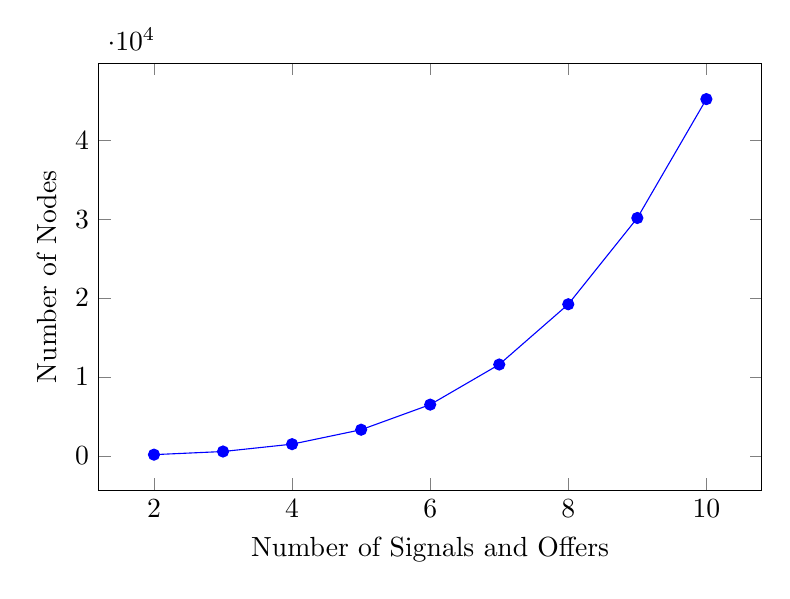
\begin{tikzpicture}
\begin{axis}[
	xlabel=Number of Signals and Offers,
	ylabel=Number of Nodes,
	width=10cm,height=7cm,
    ]

% Add values and attributes for the first plot

% Add values and attributes for the second plot
\addplot[color=blue,mark=*] coordinates {
	(2, 147)
	(3, 544)
	(4, 1477)
	(5, 3306)
	(6, 6487)
	(7, 11572)
	(8, 19209)
	(9, 30142)
	(10, 45211)
};

\end{axis}
\end{tikzpicture}

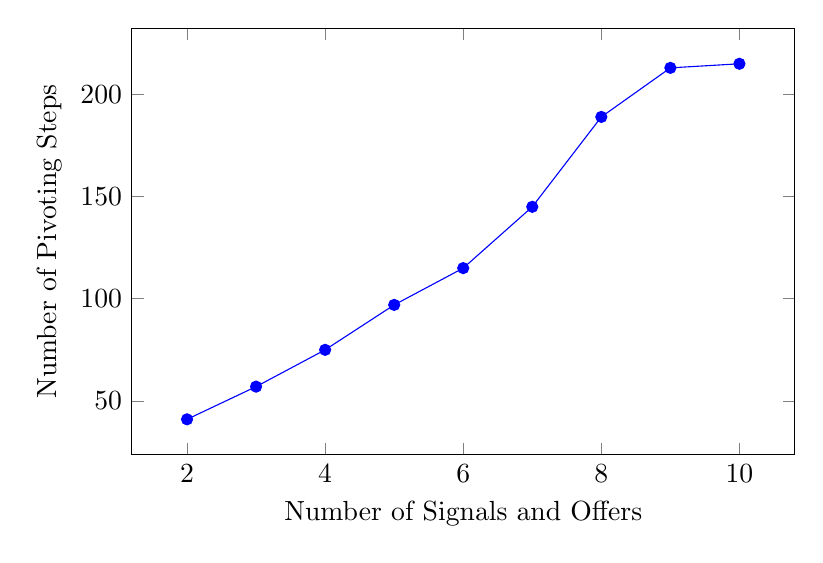
\begin{tikzpicture}
\begin{axis}[
	xlabel=Number of Signals and Offers,
	ylabel=Number of Pivoting Steps,
	width=10cm,height=7cm,
    ]

% Add values and attributes for the first plot
\addplot[color=blue,mark=*] coordinates {
	(2, 41)
	(3, 57)
	(4, 75)
	(5, 97)
	(6, 115)
	(7, 145)
	(8, 189)
	(9, 213)
	(10, 215)
};
\end{axis}
\end{tikzpicture}

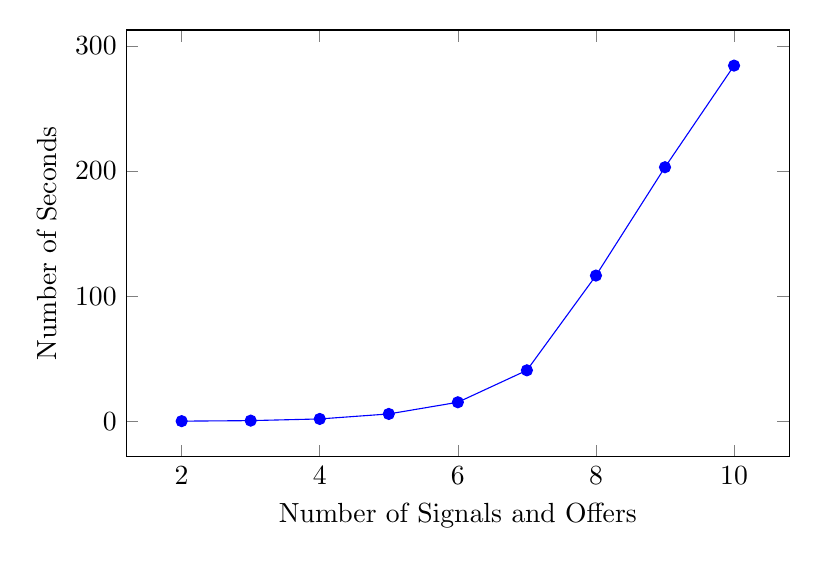
\begin{tikzpicture}
\begin{axis}[
	xlabel=Number of Signals and Offers,
	ylabel=Number of Seconds,
	width=10cm,height=7cm,
    ]

% Add values and attributes for the first plot
\addplot[color=blue,mark=*] coordinates {
	(2, 0.182)
	(3, 0.597)
	(4, 1.943)
	(5, 5.936)
	(6, 15.264)
	(7, 40.795)
	(8, 116.475)
	(9, 203.017)
	(10, 284.190)
};
\end{axis}
\end{tikzpicture}
\end{document}